\section{A Joint Perspective and Generalization of Jupyter and Active
  Documents}\label{sec:comparison}

We will now highlight the features of the ADP and Jupyter notebooks with a view towards a
possible unification of the systems.

\begin{figure}[ht]
  \documentclass[border = 120pt]{standalone}

\usepackage[landscape]{geometry}
\usepackage{tikz}
\usetikzlibrary{mindmap}
\usepackage{metalogo}
%\usepackage{dtklogos}
\usetikzlibrary{shapes, snakes}
\begin{document}
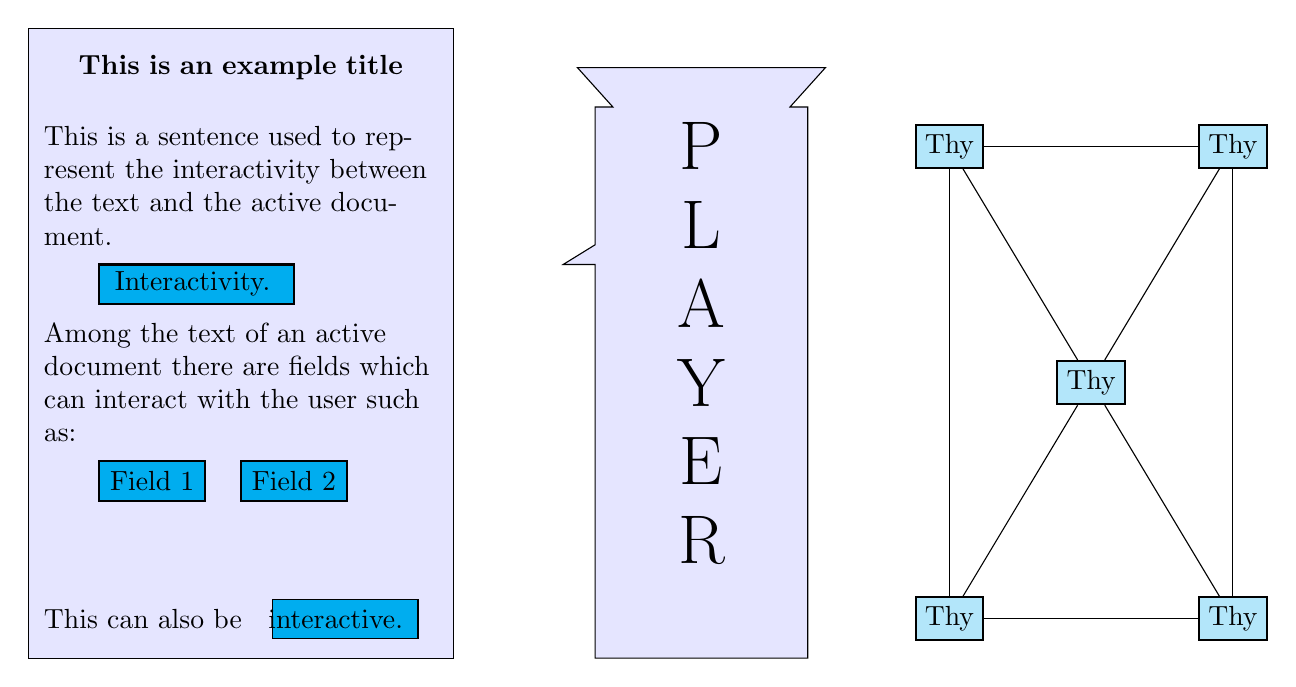
\begin{tikzpicture}[xscale=.9]

%Mother Ship
\draw[fill=blue!10] (-9,-3.5) rectangle (-15, 4.5);

%Active Document
\node[align=center, text width=5cm] at (-12,4) {\textbf{This is an example title}};
\node[align=left, text width=5cm] at (-12,2.5) {This is a sentence used to represent the interactivity between the text and the active document.};
\draw[style=thick, fill=cyan] (-14, 1.5) rectangle (-11.25, 1);
\node[align=left, text width=5cm] at (-11,1.25) {Interactivity.};

\node[align=left, text width=5cm] at (-12, 0) {Among the text of an active document there are fields which can interact with the user such as:};
\draw[style=thick, fill=cyan] (-14, -1) rectangle (-12.5, -1.5) node[pos=.5] {Field 1};
\draw[style=thick, fill=cyan] (-12, -1) rectangle (-10.5, -1.5) node[pos=.5] {Field 2};

\node[align=left, text width=5cm] at (-12,-3) {This can also be };
\draw[fill=cyan] (-11.55, -3.25) rectangle (-9.5, -2.75);
\node[align=left, text width=2cm] at (-10.5,-3) {interactive.};

% First machine
\path[draw, fill=blue!10] 
(-7, -3.5) -- 
(-7, 1.5) -- 
(-7.45, 1.5) -- 
(-7, 1.75) -- 
(-7, 3.5) -- 
(-6.75, 3.5) -- 
(-7.25, 4) -- 
(-3.75, 4) --
(-4.25, 3.5) -- 
(-4, 3.5) -- 
(-4, -3.5) -- 
cycle;

\node at (-5.5, 3) {\Huge P};
\node at (-5.5, 2) {\Huge L};
\node at (-5.5, 1) {\Huge A};
\node at (-5.5, 0) {\Huge Y};
\node at (-5.5, -1) {\Huge E};
\node at (-5.5, -2) {\Huge R};

// Nodes

\node[draw, fill=cyan!30, thick] (a) at (-2, -3) {Thy};
\node[draw, fill=cyan!30, thick] (b) at (2, -3) {Thy};
\node[draw, fill=cyan!30, thick] (c) at (2, 3) {Thy};
\node[draw, fill=cyan!30, thick] (d) at (-2, 3) {Thy};
\node[draw, fill=cyan!30, thick] (e) at (0, 0) {Thy};
\foreach \from/\to in {a/b, b/c, c/d, a/d, a/e, e/b, c/e, d/e}
\draw [-] (\from) -- (\to);

\end{tikzpicture}
\end{document}
















%%% Local Variables:
%%% mode: latex
%%% TeX-master: "report"
%%% End:

  \caption{Active Documents}\label{fig:graph2}
\end{figure}

\emph{Active Documents} need a Player process (e.g. the Planetary system) that makes them
executable, gives access to provenance and copyright/licensing information, and supports
various forms of validation. Figure~\ref{fig:graph2} shows the situation in analogy to
Figure~\ref{fig:activedocs}: On the left we see an active document -- a web page in a
browser -- as it is seen by the user: it contains text interspersed with regions that are
interactive because they have been bound to semantic services, which are executed by the
player system -- in the middle -- that interprets the represented content structures --
the mathematical knowledge; here depicted by a theory graph on the right.


In \emph{Juypther the situation is similar}, the user interacts with a dynamic web page --
the Jupyter notebook interface -- in a browser that is a mathematical text interspersed
with areas of interactivity: the computation cells. These can generate mathematical
content and righ media output into the notebook upon user request. We see the notebook
interface on the left of Figure~\ref{fig:graph3}. Again, we have a ``player process'' the
Jupyter system and displays the text from the notebook and the computational kernel that
runs the code for the notebook. Note that the notebook (source) is also a representation
of mathematical knowledge; we see it on the right of Figure~\ref{fig:graph3}.

\begin{figure}[ht]
  \documentclass[border = 120pt]{standalone}

\usepackage[landscape]{geometry}
\usepackage{tikz}
% \usetikzlibrary{mindmap}
% \usepackage{metalogo}
\usetikzlibrary{shapes, snakes}
\begin{document}
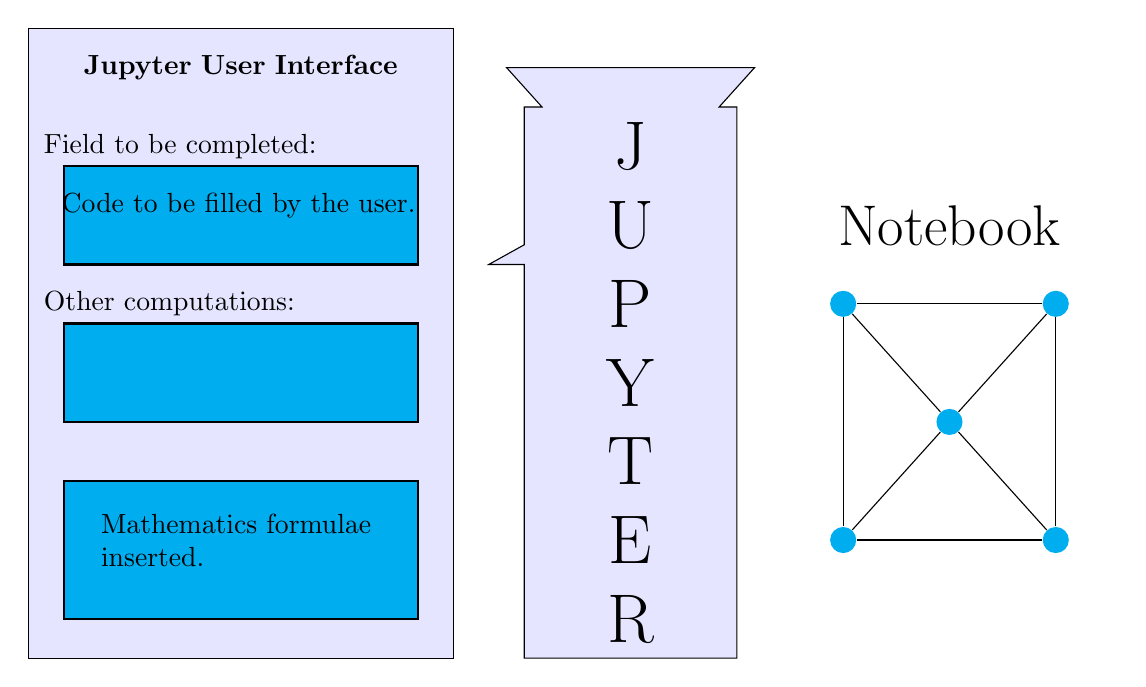
\begin{tikzpicture}[xscale=.9]

%Mother Ship
\draw[fill=blue!10] (-7,-3.5) rectangle (-13, 4.5);

%Jupyter Interface
\node[align=center, text width=5cm] at (-10,4) {\textbf{Jupyter User Interface}};
\node[align=left, text width=5cm] at (-10,3) {Field to be completed:};

%% User Interface
\draw[style=thick, fill=cyan] (-12.5, 2.75) rectangle (-7.5, 1.5);
\node[align=left, text width=5cm] at (-9.75,2.25) {Code to be filled by the user.};
\node[align=left, text width=5cm] at (-10,1) {Other computations:};
\draw[style=thick, fill=cyan] (-12.5, 0.75) rectangle (-7.5, -0.5);

\draw[style=thick, fill=cyan] (-12.5, -1.25) rectangle (-7.5, -3);
\node[align=left, text width=4cm] at (-9.75,-2) {Mathematics formulae inserted.};

% First machine
\path[draw, fill=blue!10] 
(-6, -3.5) -- 
(-6, 1.5) -- 
(-6.5, 1.5) -- 
(-6, 1.75) -- 
(-6, 3.5) -- 
(-5.75, 3.5) -- 
(-6.25, 4) -- 
(-2.75, 4) --
(-3.25, 3.5) -- 
(-3, 3.5) -- 
(-3, -3.5) -- 
cycle;

\node at (-4.5, 3) {\Huge J};
\node at (-4.5, 2) {\Huge U};
\node at (-4.5, 1) {\Huge P};
\node at (-4.5, 0) {\Huge Y};
\node at (-4.5, -1) {\Huge T};
\node at (-4.5, -2) {\Huge E};
\node at (-4.5, -3) {\Huge R};

\tikzstyle{every node} = [circle]
\node[fill=cyan] (a) at (-1.5, -2) { };
\node[fill=cyan] (b) at (1.5, -2) { };
\node[fill=cyan] (c) at (1.5, 1) { };
\node[fill=cyan] (d) at (-1.5, 1) { };
\node[fill=cyan] (e) at (0, -0.5) { };
\foreach \from/\to in {a/b, b/c, c/d, a/d, a/e, e/b, c/e, d/e}
\draw [-] (\from) -- (\to);

\node[align=center, text width=4cm] at (0,2) {\huge Notebook};

\end{tikzpicture}
\end{document}

%%% Local Variables:
%%% mode: latex
%%% TeX-master: t
%%% End:

  \caption{Jupyter Communication}\label{fig:graph3}
\end{figure}

This already hints at a synthesis of the two systems; we make this explicit in
Figure~\ref{fig:graph4}: We build a combined player system that combines the complementary
features of both systems. 

On the \emph{user interface} side this combined player 
\begin{compactenum}
\item allows free-form mathematical documents with interactivity regions like in active
  documents, but also 
\item provides computational cells with read-eval-print style interaction with dedicated
  computational machines.
\end{compactenum}
We have tried to indicate this in the mixed user interface in Figure~\ref{fig:graph3}. 

On \emph{the computational side}, it combines
\begin{compactenum}
\item the generic semantic services of the MMT Tool based with
\item dedicated computational machines running code in separate kernel processes. 
\end{compactenum}
Note that all of these need to share a notion of ``mathematical state'' so that the user
interface can present a consistent view to the user.

\begin{figure}[ht]
  \documentclass[border = 120pt]{standalone}

\usepackage[landscape]{geometry}
\usepackage{tikz}
\usetikzlibrary{shapes,snakes}
\begin{document}
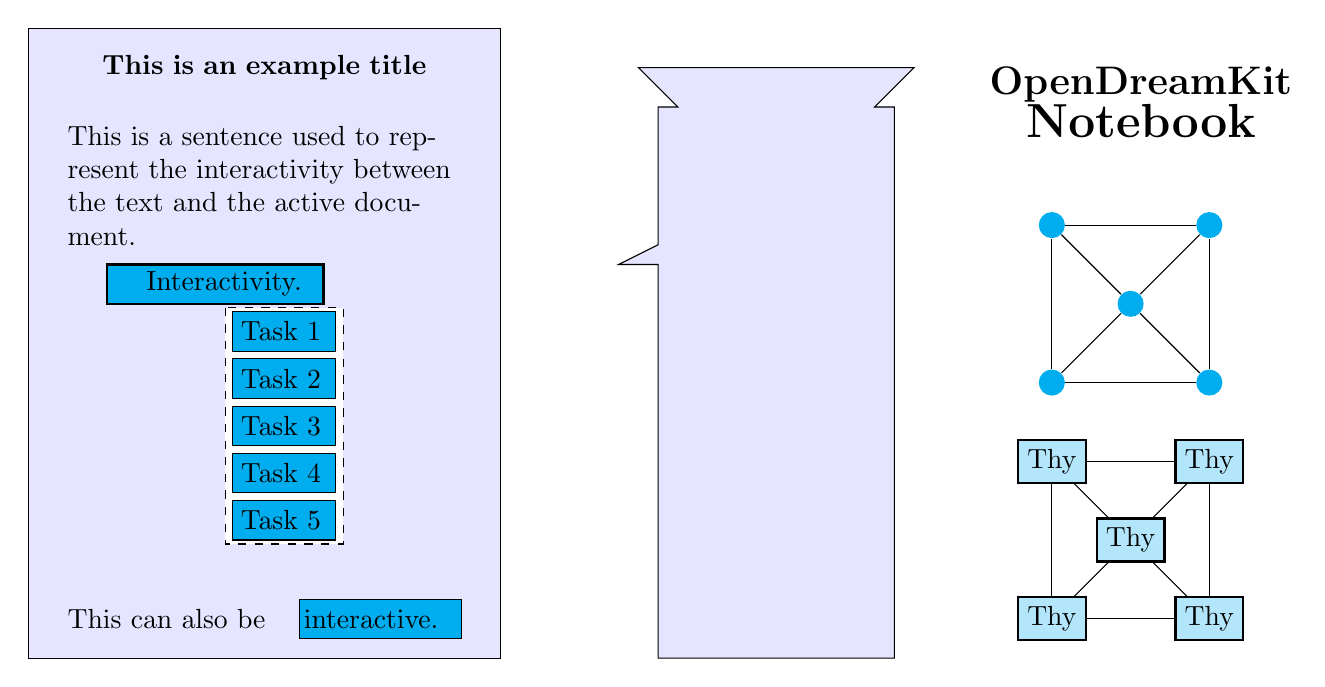
\begin{tikzpicture}

%Mother Ship
\draw[fill=blue!10] (-9,-3.5) rectangle (-15, 4.5);

%Active Document
\node[align=center, text width=5cm] at (-12,4) {\textbf{This is an example title}};
\node[align=left, text width=5cm] at (-12,2.5) {This is a sentence used to represent the interactivity between the text and the active document.};

%%Text
\draw[style=thick, fill=cyan] (-14, 1.5) rectangle (-11.25, 1);
\node[align=left, text width=5cm] at (-11,1.25) {Interactivity.};

\draw[style=dashed, fill=white] (-12.5, 0.95) rectangle (-11, -2.05);
\draw[fill=cyan] (-12.4, 0.9) rectangle (-11.1, 0.4);
\node[align=left, text width=2cm] at (-11.3,0.65) {Task 1};
\draw[fill=cyan] (-12.4, 0.3) rectangle (-11.1, -0.2);
\node[align=left, text width=2cm] at (-11.3, 0.05) {Task 2};
\draw[fill=cyan] (-12.4, -0.3) rectangle (-11.1, -0.8);
\node[align=left, text width=2cm] at (-11.3,-0.55) {Task 3};
\draw[fill=cyan] (-12.4, -0.9) rectangle (-11.1, -1.4);
\node[align=left, text width=2cm] at (-11.3,-1.15) {Task 4};
\draw[fill=cyan] (-12.4, -1.5) rectangle (-11.1, -2);
\node[align=left, text width=2cm] at (-11.3,-1.75) {Task 5};

\node[align=left, text width=5cm] at (-12,-3) {This can also be };
\draw[fill=cyan] (-11.55, -3.25) rectangle (-9.5, -2.75);
\node[align=left, text width=2cm] at (-10.5,-3) {interactive.};

% First machine
\path[draw, fill=blue!10] 
(-7, -3.5) -- 
(-7, 1.5) -- 
(-7.5, 1.5) -- 
(-7, 1.75) -- 
(-7, 3.5) -- 
(-6.75, 3.5) -- 
(-7.25, 4) -- 
(-3.75, 4) --
(-4.25, 3.5) -- 
(-4, 3.5) -- 
(-4, -3.5) -- 
cycle;


%% Jupyter Program

\node[align=center, text width=4cm] at (-1,3.5) {\textbf{\begin{tabular}{c}\Large OpenDreamKit\\\LARGE Notebook\end{tabular}}};

\node[circle,fill=cyan] (a) at (-2, 0) { };
\node[circle,fill=cyan] (b) at (0, 0) { };
\node[circle,fill=cyan] (c) at (0, 2) { };
\node[circle,fill=cyan] (d) at (-2,2) { };
\node[circle,fill=cyan] (e) at (-1, 1) { };
\foreach \from/\to in {a/b, b/c, c/d, a/d, a/e, e/b, c/e, d/e}
\draw [-] (\from) -- (\to);

\node[draw, fill=cyan!30, thick] (a) at (-2, -3) {Thy};
\node[draw, fill=cyan!30, thick] (b) at (0, -3) {Thy};
\node[draw, fill=cyan!30, thick] (c) at (0, -1) {Thy};
\node[draw, fill=cyan!30, thick] (d) at (-2, -1) {Thy};
\node[draw, fill=cyan!30, thick] (e) at (-1, -2) {Thy};
\foreach \from/\to in {a/b, b/c, c/d, a/d, a/e, e/b, c/e, d/e}
\draw [-] (\from) -- (\to);
\end{tikzpicture}
\end{document}


%%% Local Variables:
%%% mode: latex
%%% TeX-master: t
%%% End:

  \caption{Jupyter combined with Active Documents}\label{fig:graph4}
\end{figure}

The new player process relies on the availability of three ``declarative compondens'' that
also need to be in a consistent representation. 
\begin{compactenum}
\item mathematical document text 
\item theory-graph shaped content representations, and 
\item engine-specific code 
\end{compactenum}
We will call these tri-partite representations that combine the parts of Jupyter notebooks
and OMDoc documents \textbf{OpenDreamKit Notebooks}.



%%% Local Variables:
%%% mode: latex
%%% TeX-master: "report"
%%% End:
